%\documentclass[aspectratio=169]
\documentclass[aspectratio=169,xcolor=dvipsnames]{beamer}
%\usetheme{Copenhagen}
\usetheme{boxes}
\setbeamertemplate{navigation symbols}{}
\setbeamertemplate{footline}[frame number]
%\setbeamertemplate{footline}{}
\usecolortheme{dove}   %[named=black]
\usepackage{appendixnumberbeamer}
\usepackage[utf8]{inputenc}

\usepackage{graphicx}         
\graphicspath{ {./Pictures/} }
\usepackage{amsmath}
\usepackage{amsfonts}
\usepackage{amssymb}
\usepackage{amsthm}
\usepackage{mathtools}
\usepackage{commath}
\usepackage{multimedia}
\usepackage{subcaption}
\usepackage{numprint032}
\usepackage{media9}
\addmediapath{Animations/}
\newcommand{\Sta}{y}
\newcommand{\Adj}{p}
\newcommand{\Con}{u}
\begin{document}

\title[]{PDE-Constrained Optimization for Multiscale Particle Dynamics}
\author[Jonna Roden]{Jonna Roden}
\institute[UoE]{University of Edinburgh/MIGSAA\\ 
	\vspace{0.2cm}
	Joint work with Ben Goddard and John Pearson}
\date{7th April 2021}

\begin{frame}
\titlepage
\end{frame}
 
 
\begin{frame}
	\frametitle{Structure of the Talk}
	 
	 \begin{itemize}
	 	\item Part 1: Modelling (Multiscale Particle Dynamics)
	 	\item Part 2: Optimization (with PDE constraints)
	 	\item Part 3: Numerical Methods 
	 	\item Part 4: Results
	 \end{itemize}
\end{frame}


\begin{frame}
	\frametitle{Part 1: Modelling}
	\begin{columns}
		\column{0.8 \linewidth}
		Consider a particle density $\rho$ 
		on $\Sigma =  (0,T) \times \Omega$, \\ where $\partial \Sigma := (0,T) \times \partial \Omega $.
		\vspace{0.8cm}
		\textbf{\\ Diffusion, advection and \textcolor{red}{particle interactions}}
		\begin{align*}
		\partial_t \rho &= \nabla^2 \rho - \nabla \cdot (\rho \vec{w}) +\textcolor{red}{ \nabla \cdot \int_\Omega \rho(\vec{x}) \rho(\vec{x}\hspace{0.2em}') \nabla V_2(|\vec{x}-\vec{x}\hspace{0.2em}'|)d\vec{x}\hspace{0.2em}'} \qquad\text{in    } \Sigma\\
		\\
		\text{BC }& \text{and IC:}\\
		\frac{\partial \rho}{\partial n}& - \rho \vec{w} \cdot \vec{n} +\textcolor{red}{ \int_\Omega \rho(\vec{x}) \rho(\vec{x}\hspace{0.2em}')  \frac{ \partial  V_2}{\partial n}(|\vec{x}-\vec{x}\hspace{0.2em}'|)d\vec{x}\hspace{0.2em}'} = 0 \quad\ \ \qquad \qquad\text{on   } \partial \Sigma   \\
		\rho(0&,\vec{x}) = \rho_0(\vec{x}) 
		\end{align*}
		\column{0.2 \linewidth}
		\vspace{-1cm}
		\begin{figure}
			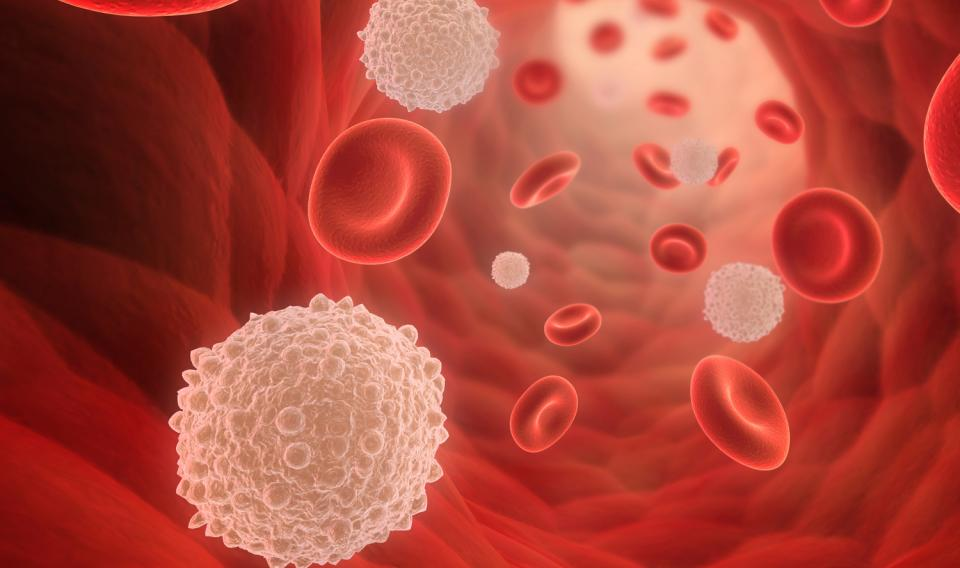
\includegraphics[width=3cm]{bloodcells.jpg}\\
			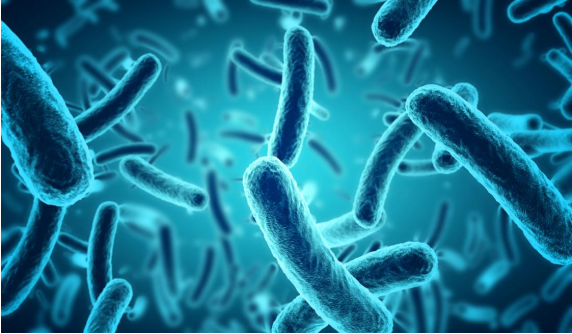
\includegraphics[width=3cm]{bacteria.png}\\
			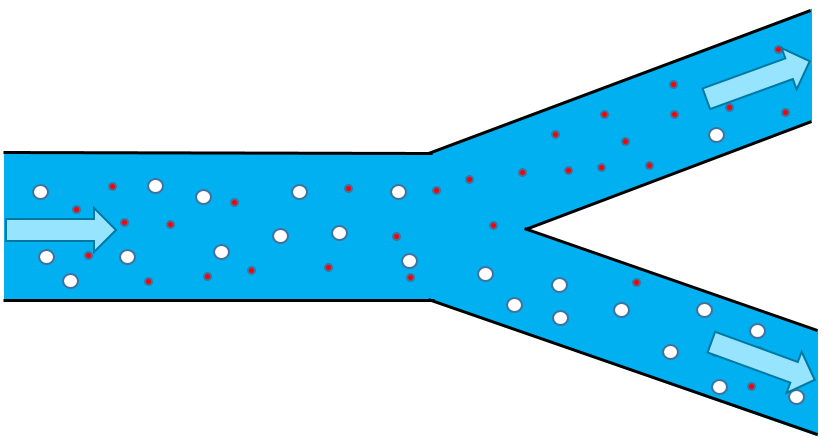
\includegraphics[width=3cm]{Microfilter.png}\\
			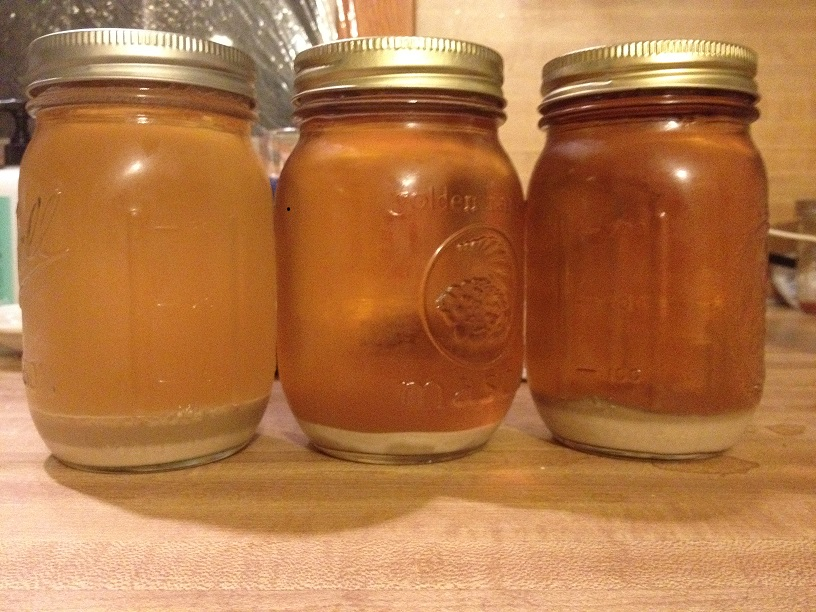
\includegraphics[width=3cm]{beer.png}
		\end{figure}
	\end{columns}
\end{frame}


\begin{frame}
	\frametitle{Part 2: Optimization}
	\begin{columns}


		\column{0.8 \linewidth}
		\begin{align*}
		&\min_{\rho,\vec{w}} \quad \frac{1}{2}\norm{\rho- \widehat{\rho}}_{L_2(\Sigma)}^2 + \frac{\beta}{2} \norm{\vec{w}}_{L_2(\Sigma)}^2\\
		\\
		&\text{subject to:}
		\\
		&\textcolor{gray}{ \partial_t \rho = \nabla^2 \rho - \nabla \cdot (\rho \vec{w})+}\textcolor{Lavender}{\nabla \cdot \int_\Omega \rho(\vec{x}) \rho(\vec{x}\hspace{0.2em}') \nabla V_2(|\vec{x}-\vec{x}\hspace{0.2em}'|)d\vec{x}\hspace{0.2em}'} \qquad \textcolor{gray}{ \text{in    } \Sigma}\\
		\\
		&\textcolor{gray}{\text{BC } \text{and IC:}}\\
		&\textcolor{gray}{\frac{\partial \rho}{\partial n} - \rho \vec{w} \cdot \vec{n} +}\textcolor{Lavender}{ \int_\Omega \rho(\vec{x}) \rho(\vec{x}\hspace{0.2em}')  \frac{ \partial  V_2}{\partial n}(|\vec{x}-\vec{x}\hspace{0.2em}'|)d\vec{x}\hspace{0.2em}'} \textcolor{gray}{= 0 \quad \ \ \qquad \qquad \text{on   } \partial \Sigma  } \\
		&\textcolor{gray}{\rho(0,\vec{x}) = \rho_0(\vec{x})} 
		\end{align*}
		\column{0.2 \linewidth}
		\vspace{-1cm}
		\begin{figure}	
			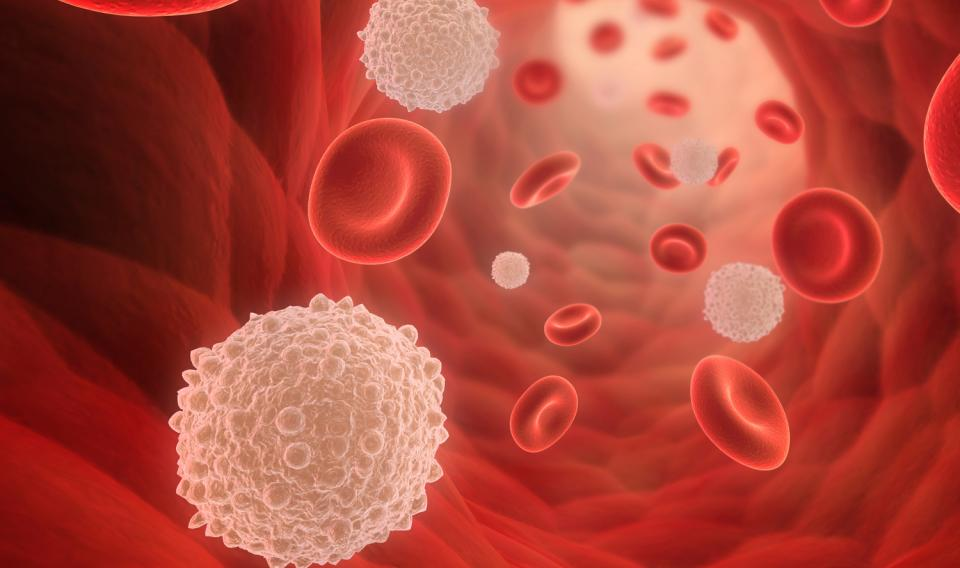
\includegraphics[width=3cm]{bloodcells.jpg}\\
			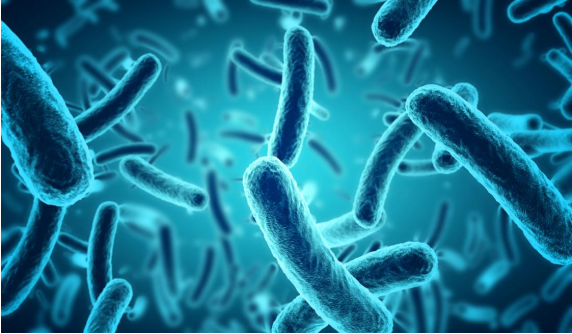
\includegraphics[width=3cm]{bacteria.png}\\			
			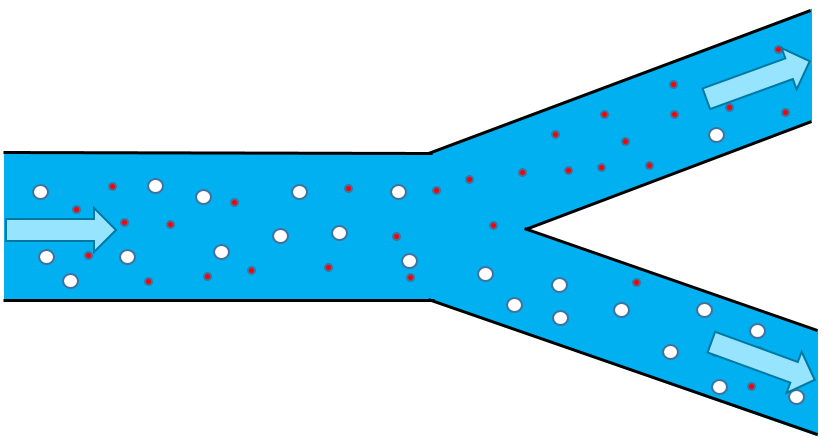
\includegraphics[width=3cm]{Microfilter.png}\\
			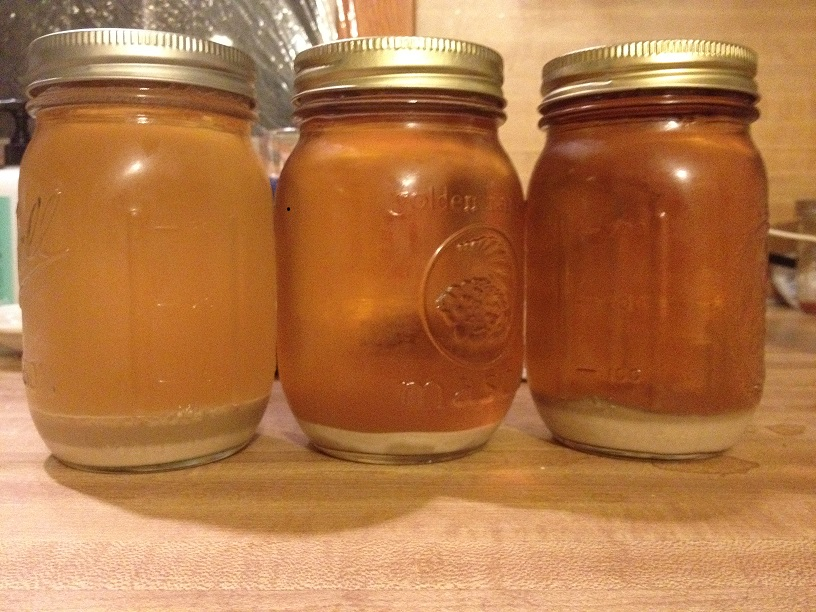
\includegraphics[width=3cm]{beer.png}
		\end{figure}
	\end{columns}
\end{frame}



\begin{frame}
	\frametitle{Part 2: Optimization}
	\textbf{The (first-order) optimality system}\\
     
	\begin{align*}
	 \partial_t \rho &= \nabla^2 \rho - \nabla \cdot (\rho \textcolor{blue}{\vec{w}})
	+ \nabla \cdot \int_\Omega \rho(\vec{x}) \rho(\vec{x}\hspace{0.2em}') \nabla V_2(|\vec{x}-\vec{x}\hspace{0.2em}'|)d\vec{x}\hspace{0.2em}'  \\
	\partial_t q &= -\nabla^2 q - \nabla q \cdot \textcolor{blue}{\vec{w}} + \int_\Omega \textcolor{ForestGreen}{\rho(\vec{x}\hspace{0.2em}')} \bigg(\nabla q(\vec{x}) + \nabla q(\vec{x}\hspace{0.2em}')\bigg)\cdot  \nabla V_2(|\vec{x}-\vec{x}\hspace{0.2em}'|)d\vec{x}\hspace{0.2em}' \\
    \textcolor{blue}{\vec{w}} \ &= - \frac{1}{\beta}\textcolor{ForestGreen}{\rho} \nabla  \textcolor{red}{q}\\
    \\
    \rho(0,\vec{x})&=\rho_0(\vec{x}), \qquad q(T,\vec{x})= 0, \qquad \qquad \text{+BCs}\\
	\end{align*}
\end{frame}

\begin{frame}
	\frametitle{Part 2: Optimization}
     \textbf{Problem:} Negative diffusion term in $q$ causes numerical instability.\\
     \textbf{Solution:} Change of time variable for this PDE: $\textcolor{magenta}{\tau = T-t}$.
	\begin{align*}
	\partial_t \rho (t,\vec{x}) &= \nabla^2 \rho (t,\vec{x}) - \nabla \cdot (\rho(t,\vec{x}) \vec{w}(t,\vec{x}) )
	+ \nabla \cdot \int_\Omega \rho(t,\vec{x}) \rho(t,\vec{x}\hspace{0.2em}') \nabla V_2(|\vec{x}-\vec{x}\hspace{0.2em}'|)d\vec{x}\hspace{0.2em}'  \\
	\partial_{\textcolor{magenta}{\tau}} q(\textcolor{magenta}{\tau},\vec{x})  &= \nabla^2 q(\textcolor{magenta}{\tau},\vec{x})  + \nabla q(\textcolor{magenta}{\tau},\vec{x})  \cdot \vec{w}(\textcolor{magenta}{\tau},\vec{x})  \\
	&- \int_\Omega \textcolor{ForestGreen}{\rho(}\textcolor{magenta}{\tau}\textcolor{ForestGreen}{, \vec{x}\hspace{0.2em}')} \bigg(\nabla q(\textcolor{magenta}{\tau}, \vec{x} ) + \nabla q(\textcolor{magenta}{\tau},\vec{x}\hspace{0.2em}')\bigg) \cdot \nabla V_2(|\vec{x}-\vec{x}\hspace{0.2em}'|)d\vec{x}\hspace{0.2em}' \\
    \vec{w}(t,\vec{x}) \ &= - \frac{1}{\beta}\rho(t,\vec{x}) \nabla q(t,\vec{x}) \\
    \\
	\rho(0,\vec{x})&=\rho_0(\vec{x}), \qquad q(\textcolor{magenta}{0},\vec{x})= 0, \qquad \qquad \text{+BCs}
	\end{align*}
\end{frame}


\begin{frame}
	\frametitle{Part 3: Numerical Methods}

	\begin{itemize} 
		\item Challenge 1: Particle interaction term is nonlinear and nonlocal (+ nonlocal BCs).
		\\How to avoid shortcomings of standard methods (FEM/FDM)?\\
		\vspace{0.3 cm}		
		\textbf{$\Rightarrow$ Pseudospectral methods}		
		\vspace{0.2 cm}
		\item Challenge 2: One PDE is forward in time, the other backward. \\How to do time stepping?\\
		\vspace{0.3 cm}	
		\textbf{$\Rightarrow$ Fixed point algorithm}
	\end{itemize}

\end{frame}


\begin{frame}
	\frametitle{Part 3: Numerical Methods}
	\textbf{Pseudospectral Methods}\\
	\vspace{0.3 cm}
    \begin{itemize}
    	\item Reduce both PDEs to systems of ODEs.
    	\item Discretize time (accurate interpolation).
    	\item Equations can now be solved using a DAE solver (when given all necessary inputs).
    \end{itemize}
	
\end{frame}


\begin{frame}
	\frametitle{Part 3: Numerical Methods}
\textbf{Fixed point algorithm}\\
\vspace{0.4 cm}
Initialize with guess $\textcolor{blue}{\vec{w}^{(0)}}$.
	\begin{enumerate}
     \item 
     Solve $\displaystyle \partial_t \rho  = \nabla^2 \rho  - \nabla \cdot (\rho \textcolor{blue}{\vec{w}^{(i)}} )
     + \nabla \cdot \int_\Omega \rho(\vec{x}) \rho(\vec{x}\hspace{0.2em}') \nabla V_2(|\vec{x}-\vec{x}\hspace{0.2em}'|)d\vec{x}\hspace{0.2em}'. 
     $
	 \item
     Solve $\displaystyle \partial_{{\tau}} q  = \nabla^2 q  + \nabla q  \cdot \textcolor{blue}{\vec{w}^{(i)}}  
     - \int_\Omega \textcolor{ForestGreen}{\rho^{(i)}(\vec{x}\hspace{0.2em}')} \bigg(\nabla q( \vec{x} ) + \nabla q( \vec{x}\hspace{0.2em}')\bigg) \cdot \nabla V_2(|\vec{x}-\vec{x}\hspace{0.2em}'|)d\vec{x}\hspace{0.2em}'. 
     $
     \item Solve $\displaystyle \textcolor{blue}{\vec{w}^{(i)}_g} = - \frac{1}{\beta}\textcolor{ForestGreen}{{\rho}^{(i)}} \nabla \textcolor{red}{{q}^{(i)}}.$
     \vspace{0.4 cm}
     \item Measure the error: $ \mathcal{E} = ||\textcolor{blue}{\vec{w}^{(i)}} - \textcolor{blue}{\vec{w}^{(i)}_g}||$.
     \vspace{0.2 cm}
	 \item Update control, with $\lambda \in [0,1]$:       $\quad \textcolor{blue}{\vec{w}^{(i+1)}} = (1-\lambda)\textcolor{blue}{\vec{w}^{(i)}} + \lambda \textcolor{blue}{\vec{w}^{(i)}_g}.$	 
	\end{enumerate}	
\vspace{0.2 cm}
Iterate until $\mathcal{E} <TOL$.
\end{frame}




\begin{frame}
	\frametitle{Part 4: Results}
	\begin{columns}
	
	
	\column{0.8 \linewidth}
	\textbf{Reminder: The Optimization Problem}
	\begin{align*}
		&\min_{\rho,\vec{w}} \quad \frac{1}{2}\norm{\rho- \widehat{\rho}}_{L_2(\Sigma)}^2 + \frac{\beta}{2} \norm{\vec{w}}_{L_2(\Sigma)}^2\\
		\\
		&\text{subject to:}
		\\
		&\textcolor{gray}{ \partial_t \rho = \nabla^2 \rho - \nabla \cdot (\rho \vec{w})+}\textcolor{Lavender}{\nabla \cdot \int_\Omega \rho(\vec{x}) \rho(\vec{x}\hspace{0.2em}') \nabla V_2(|\vec{x}-\vec{x}\hspace{0.2em}'|)d\vec{x}\hspace{0.2em}'} \qquad \textcolor{gray}{ \text{in    } \Sigma}\\
		\\
		&\textcolor{gray}{\text{BC } \text{and IC:}}\\
		&\textcolor{gray}{\frac{\partial \rho}{\partial n} - \rho \vec{w} \cdot \vec{n} +}\textcolor{Lavender}{ \int_\Omega \rho(\vec{x}) \rho(\vec{x}\hspace{0.2em}')  \frac{ \partial  V_2}{\partial n}(|\vec{x}-\vec{x}\hspace{0.2em}'|)d\vec{x}\hspace{0.2em}'} \textcolor{gray}{= 0 \quad \ \ \qquad \qquad \text{on   } \partial \Sigma  } \\
		&\textcolor{gray}{\rho(0,\vec{x}) = \rho_0(\vec{x})} 
	\end{align*}
	\column{0.2 \linewidth}
	\vspace{-1cm}
	\begin{figure}	
		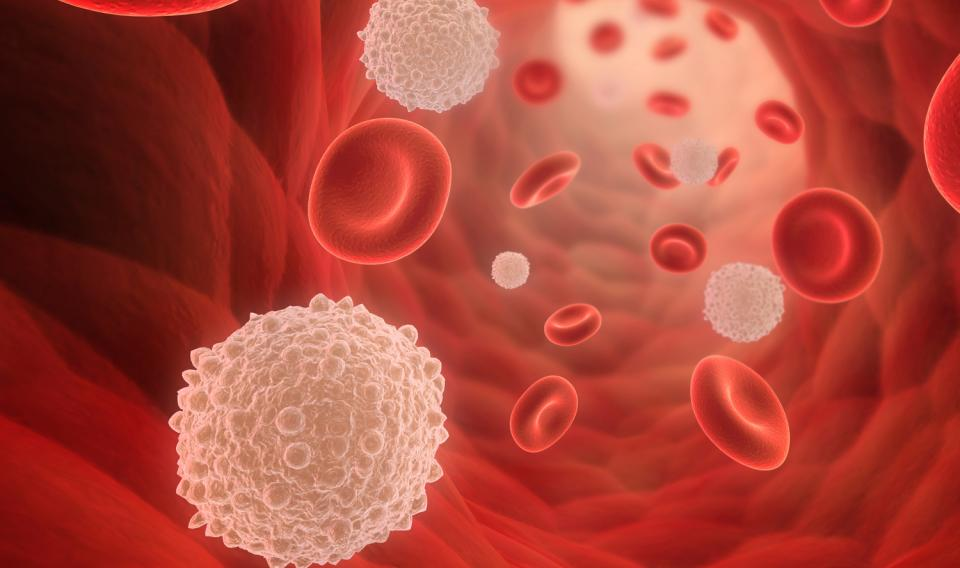
\includegraphics[width=3cm]{bloodcells.jpg}\\
		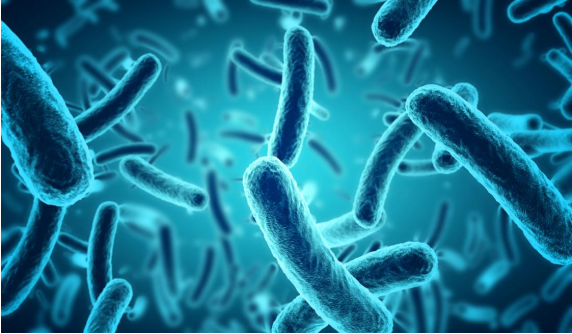
\includegraphics[width=3cm]{bacteria.png}\\			
		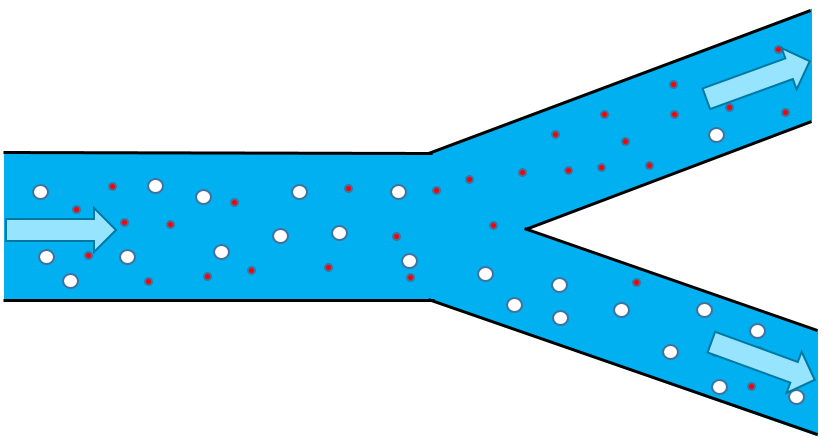
\includegraphics[width=3cm]{Microfilter.png}\\
		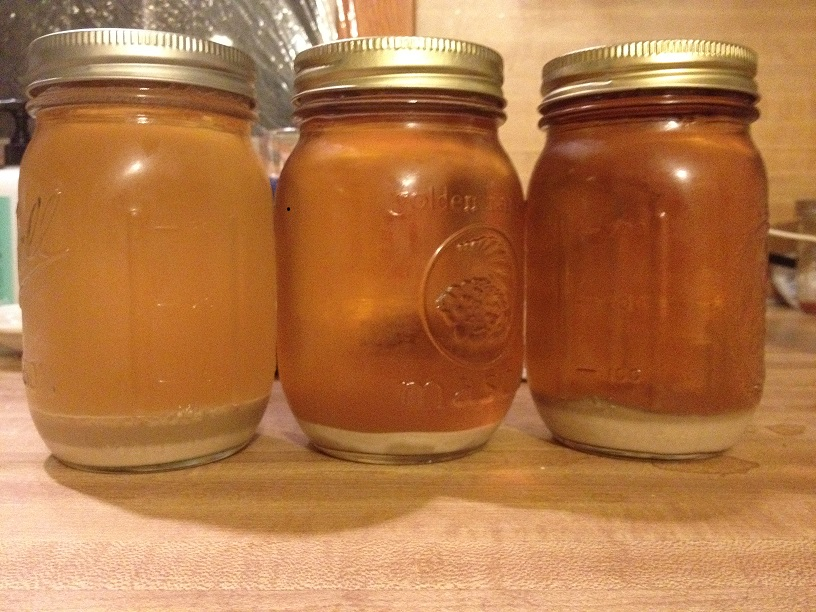
\includegraphics[width=3cm]{beer.png}
	\end{figure}
\end{columns}
\end{frame}

\begin{frame}
	\frametitle{Part 4: Results}
	Overall Cost: $\mathcal J = \frac{1}{2}\norm{\rho- \widehat{\rho}}_{L_2(\Sigma)}^2 + \frac{\beta}{2} \norm{\vec{w}}_{L_2(\Sigma)}^2$, $\mathcal J_{\vec{w}= \vec 0} = 0.0130$.

	\begin{figure}
		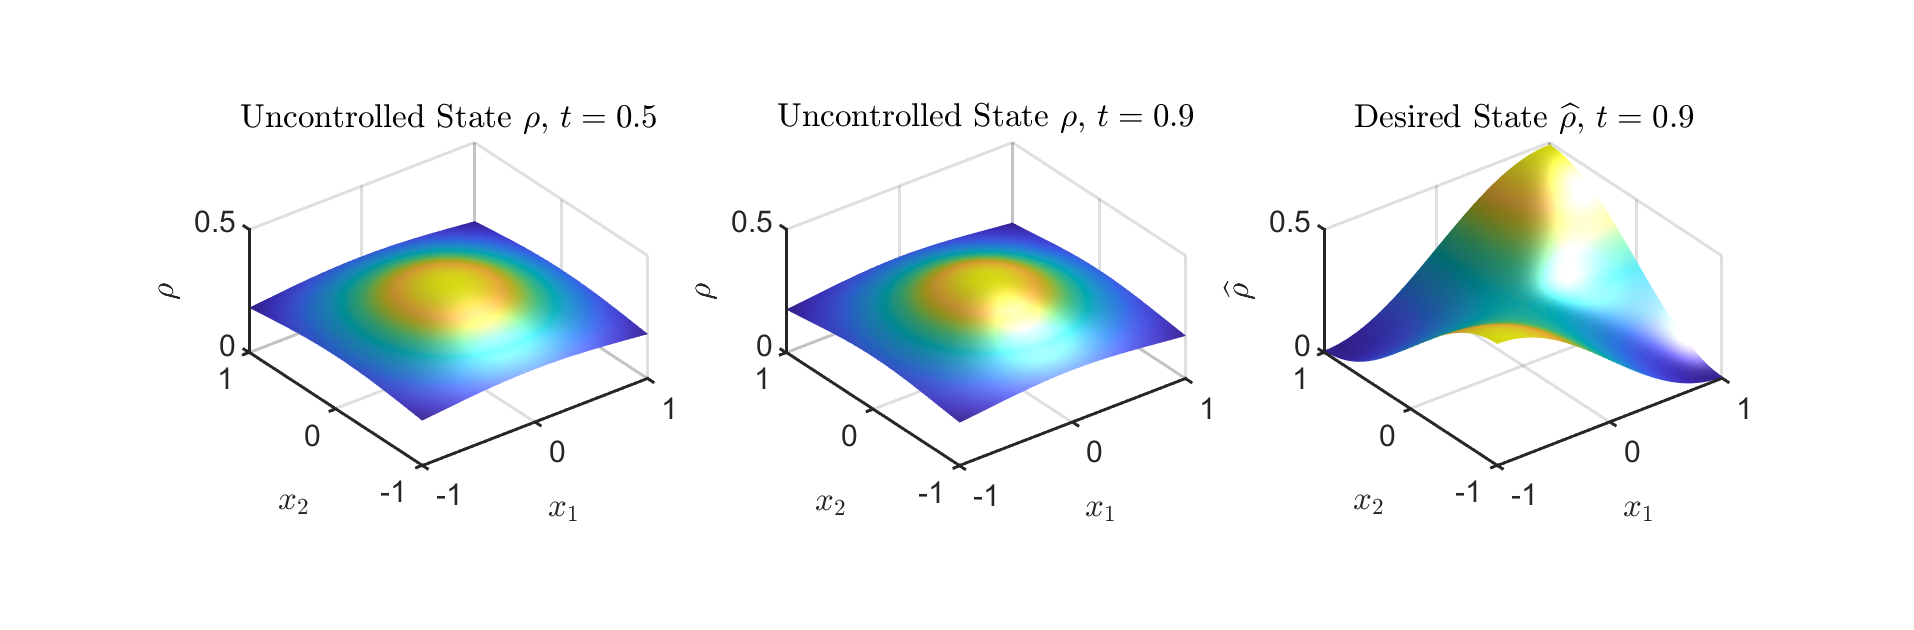
\includegraphics[width=15cm]{Res1Ex2.png}
	\end{figure}
	
\end{frame}

\begin{frame}
	\frametitle{Part 4: Results}
	\vspace{0.3cm}
	Overall Cost: $\mathcal J = \frac{1}{2}\norm{\rho- \widehat{\rho}}_{L_2(\Sigma)}^2 + \frac{\beta}{2} \norm{\vec{w}}_{L_2(\Sigma)}^2$, $\mathcal J_{\vec{w} = \vec 0} = 0.0130$, $\mathcal J_{opt} = 7.2994 \times 10^{-4}$.
	\begin{figure}
		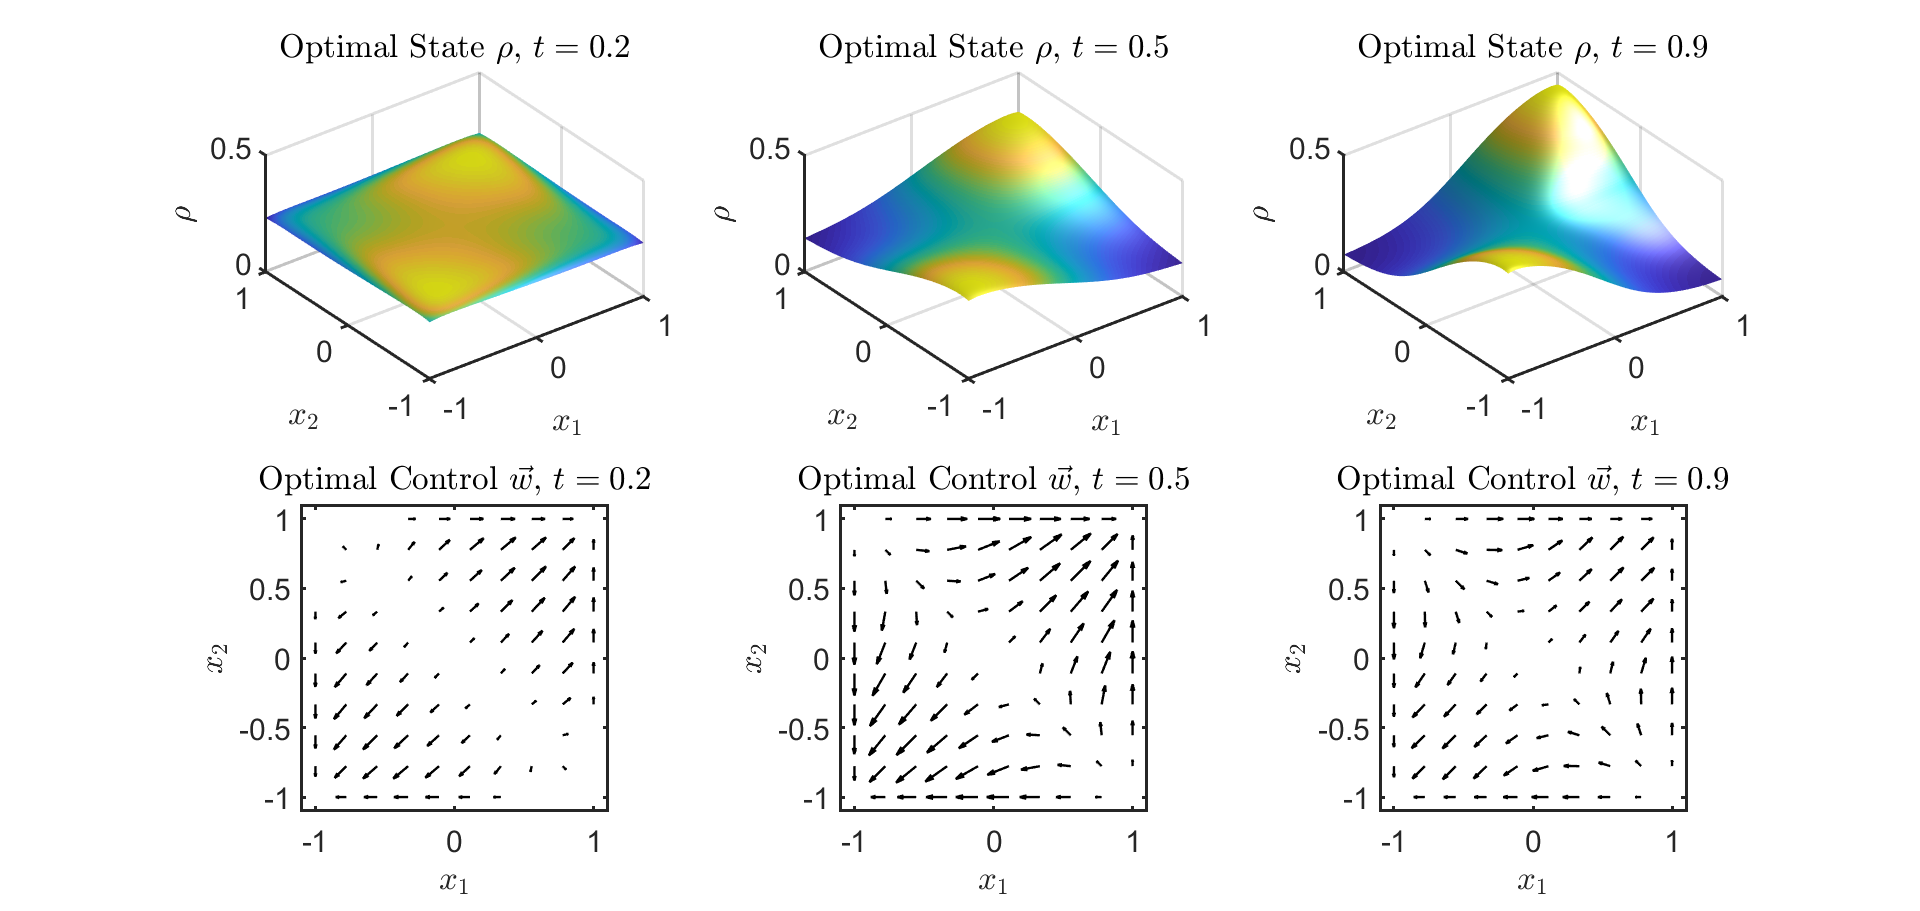
\includegraphics[width=14cm]{Res2Ex2.png}
	\end{figure}
\end{frame}




\begin{frame}
	\frametitle{Current work}
	\begin{figure}
		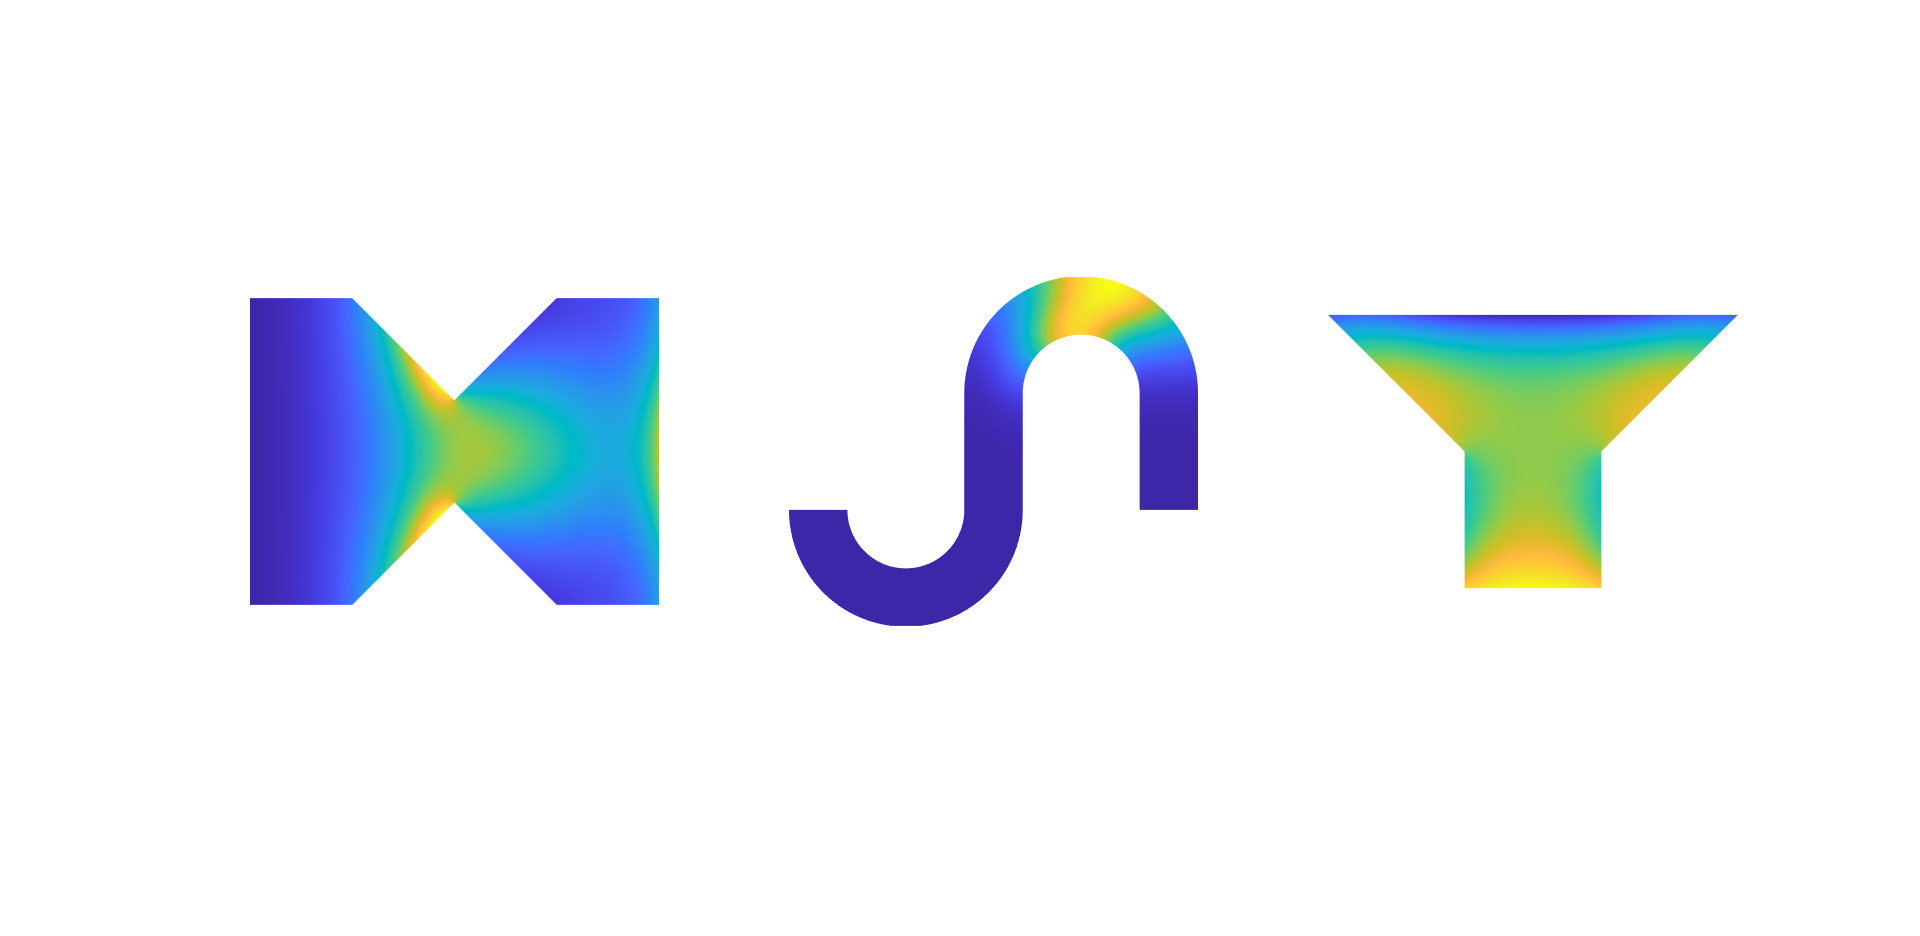
\includegraphics[width=15cm]{Future.png}
		\caption{Change to nicer images}
	\end{figure}
\end{frame}
\begin{frame}
	\frametitle{Next steps}
	\textbf{Industrial partners of the PhD}
	\begin{columns}
		\column{0.5 \linewidth}
		\begin{figure}
			
\includegraphics[width=5cm]{ufraction8.png}
			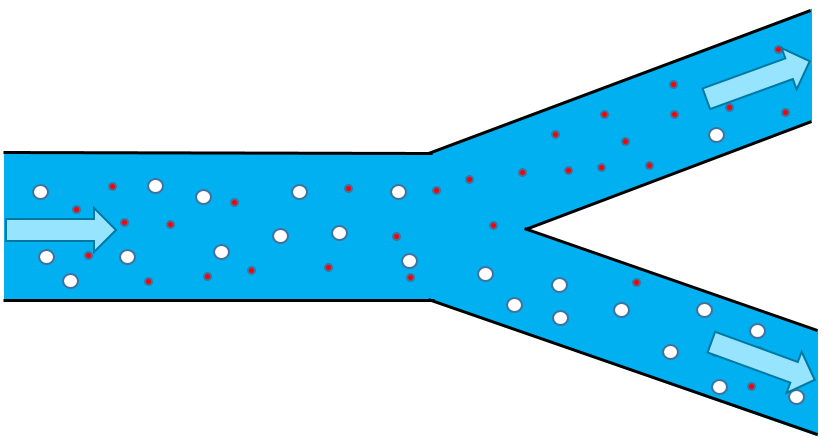
\includegraphics[width=5cm]{Microfilter.png}
			%\caption{Nanofiltration Device}
		\end{figure}
		
		\column{0.5 \linewidth}
		\begin{figure}
			
\includegraphics[width=3cm]{west.png}\\
			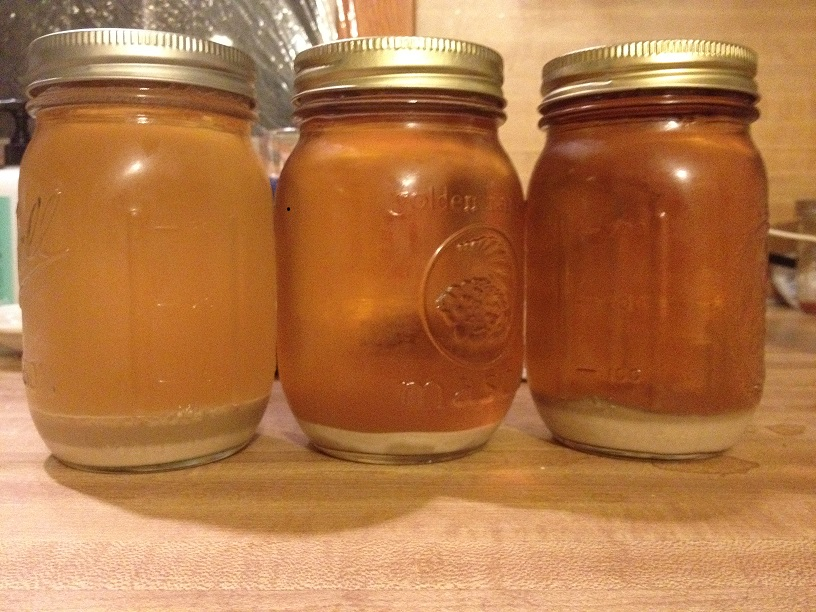
\includegraphics[width=3.5cm]{beer.png}
			%\caption{Yeast Sedimentation in Beer}
		\end{figure}
	\end{columns}
\end{frame}

\begin{frame}
	\frametitle{Summary}
	Up to now:
	\begin{itemize}
		\item Deriving PDE-constrained optimization models.
		\item Developing a suitable numerical method to solve them.
	\end{itemize}
	Current:
	\begin{itemize}
		\item Complex domains.
		\item Extended models (e.g. sedimentation, multiple species).
		\item Different boundary conditions.
	\end{itemize}
	Up next:
	\begin{itemize}
		\item Application of the method to other extended models.
		\item Application of the numerical framework to industrial processes.
	\end{itemize}
	
\end{frame}

\appendix

\begin{frame}
\frametitle{References}    
\begin{thebibliography}{10}    

	\bibitem{Us2020}
	M. Aduamoah, B. D. Goddard, J. W. Pearson and J. C. Roden.
	\newblock {\em PDE-constrained optimization models and pseudospectral methods for multiscale particle dynamics.} 
	\newblock { \em Preprint, 2020.}
	
	\bibitem{Burger1}
	M. Burger, M. Di Francesco, P.A. Markowich and  M.-T. Wolfram. 
	\newblock {\em Mean field games with nonlinear mobilities in pedestrian dynamics.}
	\newblock { \em Discrete and Continuous Dynamical Systems - Series B,} 19(5), 1311-1333, 2014. 	
	
	\bibitem{Autor1990}
	A. Nold, B.D. Goddard, P. Yatsyshin, N. Savva and S. Kalliadasis. 
	\newblock {\em 	Pseudospectral methods for density functional theory in bounded and unbounded domains}.
	\newblock {\em Journal of Computational Physics}, 334, 639-664, 2017.
	\newblock \url{https://datashare.is.ed.ac.uk/handle/10283/2647} (2DChebClass)
\end{thebibliography}
\end{frame}
\begin{frame}
	\frametitle{References: Figures}   
	\begin{thebibliography}{10}    
		
		\bibitem{F1}
		Bacteria. Digital Image.\newblock {\em USCNews.} 12 February 2008, \url{https://news.usc.edu/135660/how-bacteria-adapt-to-hostile-environments/}

		\bibitem{F2}
		Red and White Bloodcells. Digital Image.\newblock {\em The Franklin Institute. } \url{https://www.fi.edu/heart/white-blood-cells}

		\bibitem{F3}
		ufraction8 Logo. Digital Image. \newblock{ \em www.ufraction8.}
		\url{ufraction8.com}
		
		\bibitem{F4}
		WEST Logo. Digital Image. \newblock{\em WEST Brewery} \url{www.westbeer.com}
	\end{thebibliography}	
\end{frame}

\begin{frame}
	\frametitle{Part 4: Results}
	\begin{table}
\begin{tabular}{ ||c|| c | c | c | c | c ||}
\hline
& & $\beta = 10^{-3}$ & $\beta = 10^{-1}$ & $\beta = 10^{1}$ & $\beta = 10^{3}$  \\
\hline
 & $\mathcal J_{\vec w = \vec 0}$ & $0.0113$ & $0.0113$ & $0.0113$ & $0.0113$ \\
$\kappa= -1$  & $\mathcal J_{Opt}$ & $0.0013$ & $0.0104$ & $0.0113$ & $0.0113$ \\
& $\text{Iterations}$ & $676$ & $700$ & $290$ & $1$ \\
\hline
\end{tabular}
\caption{Results for the test problem, with different $\beta$}
\label{TabS5:Prob12D}
\end{table}
\end{frame}
\begin{frame}
	\frametitle{Part 2: Optimization}
	\textbf{Deriving (first-order) optimality conditions}\\
	Define the Lagrangian $\mathcal{L}(\rho, \vec{w}, q)$:
	\begin{align*}
		\mathcal{L}(\rho, \vec{w},q)&= \frac{1}{2}\norm{\rho- \widehat{\rho}}_{L_2(\Sigma)}^2 + \frac{\beta}{2} \norm{\vec{w}}_{L_2(\Sigma)}^2\\
		&+ \int_\Sigma q \textcolor{gray}{\bigg( \partial_t \rho - \nabla^2 \rho + \nabla \cdot (\rho \vec{w})
			-}\textcolor{Lavender}{ \nabla \cdot\int_\Omega \rho(\vec{x}) \rho(\vec{x}\hspace{0.2em}') \nabla V_2(|\vec{x}-\vec{x}\hspace{0.2em}'|)d\vec{x}\hspace{0.2em}'}  \textcolor{gray}{  \bigg)} d\vec{x} dt\\
		&+ \int_{\partial \Sigma} q \textcolor{gray}{ \bigg(\frac{\partial \rho}{\partial n} - \rho \vec{w} \cdot \vec{n} + }\textcolor{Lavender}{ \int_\Omega \rho(\vec{x}) \rho(\vec{x}\hspace{0.2em}')  \frac{ \partial  V_2}{\partial n}(|\vec{x}-\vec{x}\hspace{0.2em}'|)d\vec{x}\hspace{0.2em}'} \textcolor{gray}{\bigg)} d\vec{x} dt\\
	\end{align*}
	1. Take derivatives of $\mathcal{L}(\rho, \vec{w}, q)$ with respect to $\rho$, $\vec{w}$ and $q$. \\
	2. Set derivatives to zero to find stationary points. \\
\end{frame}
\end{document}